%%%%%%%%%%%%%%%%%%%%
%                 File Experiment01.tex        %
%                 Experiment M-1               %
%                   Force Table                %
%                                              %
%%%%%%%%%%%%%%%%%%%%

\labChapter{M}{Force Table with 3 Vectors at Equilibrium}
\label{lab:M1}

% Introduction
%\section{Introduction}
















\section{Background}

\textbf{OVERALL GOALS:}
Use a ``force table" to study:
\begin{enumerate}
\item[$\triangleright$] how vectors are added
\item[$\triangleright$] the concept of force vectors in equilibrium
\end{enumerate}


There are two types of physical quantities: \textbf{\textit{scalars}} and \textbf{\textit{vectors}}. The number of attributes required to define a scalar and a vector distinguishes them. A \textbf{\textit{scalar}} has just a \textbf{magnitude} telling us how large or small something is (or positive or negative); an example of a scalar quantity is temperature or speed ($\meter\per\second$)

A \textbf{\textit{vector}}, meanwhile, is a quantity that is described by both a \textbf{magnitude} \textbf{\textit{and}} \textbf{direction}. Examples of vectors are velocity (speed but with a direction; $\meter\per\second$ at some angle) or force (a push or pull on an object with a specific magnitude at some direction).

A force example: a force may be $100\,\newton$ in magnitude with direction $90\degree$ counterclockwise from the $x$-axis. This force vector is written as $100\,\newton \ @ \ 90\degree$. We will use bold face type to indicate a vector ($\vec{F_i}$) while the regular typeface will indicate scalar magnitudes and the components of a vector ($F_i$).

When several vectors act on an object, it is generally desirable to determine the sum of these vectors, called the \textbf{resultant vector}. Suppose force vectors $\vec{F}_1$ and $\vec{F}_2$ act on a body. The resultant $\vec{R}$ is defined by the vector sum of the two forces, thus
\begin{equation}
   \vec{R} = \vec{F}_1 + \vec{F}_2.
\end{equation}
If many forces act on the body, then we sum all the forces together
\begin{equation}
  \vec{R} = \sum_{i=1}^N \vec{F}_i.
\end{equation}
The resultant force is a single force which can completely represent a number of individual forces acting.  When the resultant force is zero, the object is said to be in equilibrium.

\pagebreak

There are two methods of vector addition to consider:
\begin{enumerate}
\item[$\triangleright$] The graphical method (reviewed here, but not conducted during lab today)
\item[$\triangleright$] The method of components (conducted during lab today)
\end{enumerate}

\subsection{Graphical Method}

Vectors $\vec{F}_1$ and $\vec{F}_2$  (Fig.~\ref{M01Fig01}) are added graphically as follows:
Beginning at a convenient point on a piece of graph paper, usually at the origin of a rectangular coordinate system draw one of the vectors as an arrow to scale and pointing in the proper direction.  Place the second vector with its tail at the tip of the first, again drawn to scale and pointing in the proper direction.  The resultant $\vec{R}$ is the vector drawn from the tail of the first vector to the tip of the second.  The process is illustrated in Fig.~\ref{M01Fig02} demonstrating the addition operation does not depend on the order of addition.  Thus, like scalar addition,
\begin{equation}
  \vec{F}_1 + \vec{F}_2 = \vec{F}_2 + \vec{F}_1 = \vec{R}.
\end{equation}

%Figure01
\begin{figure}[ht]
  \begin{center}        
    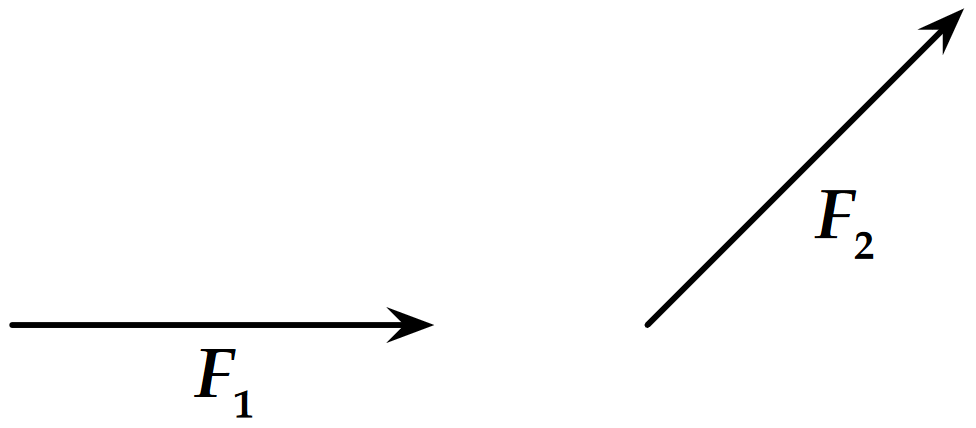
\includegraphics[width=2.2in]{Fall/Experiment01Figures/M1_ForceTable_01.png}
  \end{center}
  \caption{Two force vectors $\vec{F}_1$ and $\vec{F}_2$}
  \label{M01Fig01}  % the \label command comes AFTER the caption
\end{figure}


%Figure02
\begin{figure}%[ht]
  \begin{center}
    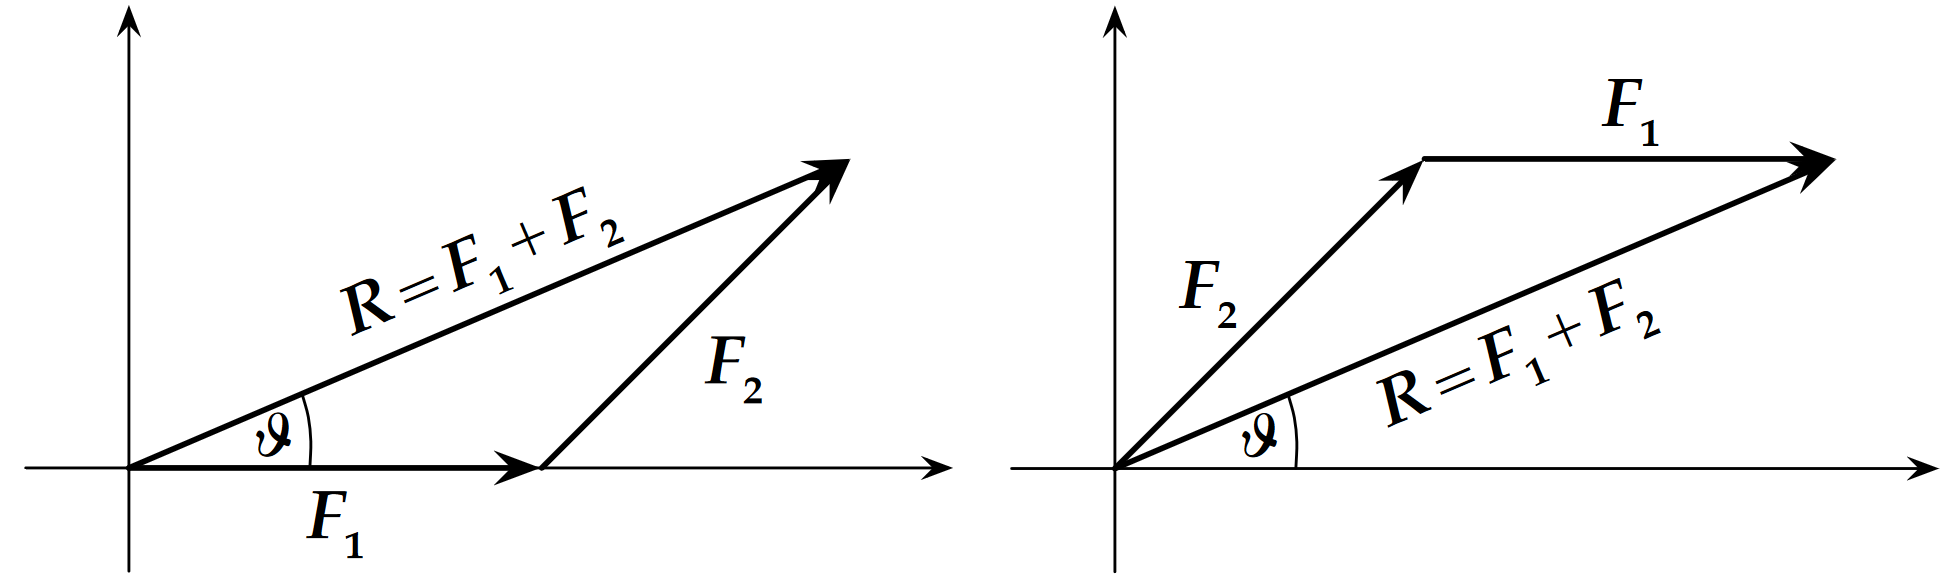
\includegraphics[width=5.6in]{Experiment01Figures/M1_ForceTable_02.png}
  \end{center}
  \caption{Adding 2 vectors $\vec{F}_1$ and $\vec{F}_2$, using the graphical (``tail-to-tip'') method.}
  \label{M01Fig02}
\end{figure}

It is important that an appropriate scale be selected with which the vectors are drawn (e.g.\ $1\,\newton = 10\,\centi\meter$). The magnitude of $\vec{R}$ is determined using a ruler, and the angle $\theta$ is measured using a protractor.  Since the negative of a vector is merely the vector pointing in the opposite direction, subtraction is addition with the negative vector pointing in the opposite direction.  Errors can be significantly reduced by using a scale that makes the drawing as large as possible. Neatness counts!

% Method of Components
\subsection{Method of Components}

The method of components is a much more useful and quantitatively accurate method of vector addition.  Each vector is resolved into components along the $x-$ and $y$-axes. That is to say, the vector addition of the two components of the vector is the vector itself.  Thus if two vectors are to be added, we add the components along each axis to form the components of the resultant.

%Figure03
\begin{figure}[ht]
  \begin{center}
    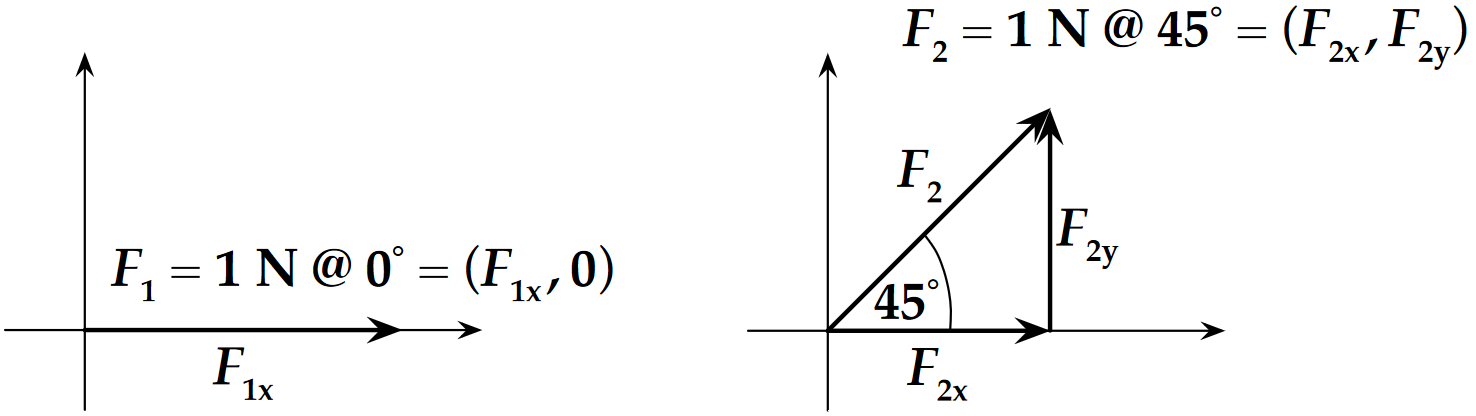
\includegraphics[width=5.6in]{Fall/Experiment01Figures/M1_ForceTable_03.png}
  \end{center}
  \caption{Adding 2 vectors $\vec{F}_1$ and $\vec{F}_2$ using the method of components. }
  \label{M01Fig03}
\end{figure}

In Fig.~\ref{M01Fig03}, the magnitudes and directions are shown for the two force vectors $\vec{F}_1$ and $\vec{F}_2$ . The magnitudes of the $x$ and $y$ components are calculated for this example as follows:
\begin{equation}
\label{Eq:M1_cosSinAngle}
  \begin{aligned} %
    F_{1,x} & = F_1 \, \cos(\theta_{1}) & \qquad F_{2,x} & = F_2 \, \cos(\theta_{2}) \\
            & = 1\,\newton\ \cos(0\degree) = 1\,\newton & &  = 1\,\newton\ \cos(45\degree) = 0.707\,\newton \\
    F_{1,y} & = F_1 \,\sin(\theta_1) & \qquad F_{2,y} & = F_2 \,\sin(\theta_2) \\
            & = 1\,\newton\ \sin(0\degree) = 0\,\newton & &  = 1\,\newton\ \sin(45\degree) = 0.707\,\newton.
  \end{aligned}
\end{equation}
Next, add the $x$-components
\[
  \vec{R}_x = F_{1,x} + F_{2,x} = 1\,\newton + 0.707\,\newton = 1.707\,\newton.
\]
Then, add the $y$-components
\[
  \vec{R}_y = F_{1,y} + F_{2,y} = 0\,\newton + 0.707\,\newton = 0.707\,\newton.
\]
The magnitude of the resultant is found using the relation
\begin{equation}
\label{Eq:M1_resultantMag}
	\vec{R}^2 = {\vec{R}_x}^2 + {\vec{R}_y}^2,
\end{equation}
or
\[
  \vec{R} = \sqrt{\left(1.707\,\newton\right)^2 +
    \left(0.707\,\newton\right)^2} = 1.848\,\newton.
\]
The angle $\theta$ specifies the direction of the resultant and it can be calculated by noting that
\begin{equation}
  \tan\theta = R_{y} / R_{x}
\end{equation}
and
\begin{align} %
\label{Eq:M1_arctan}
  \theta = \arctan (R_{y} / R_{x}).
\end{align}

For this example illustrated in Fig.~\ref{M01Fig04}
\begin{align} %
  \tan \theta = (0.707\,\newton) / (1.707\,\newton) = 0.414\,\newton,
\end{align}
\begin{align} %
  \theta = \arctan(0.414) = 22.5\degree.
\end{align}

%Figure04
\begin{figure}[h]
  \begin{center}
    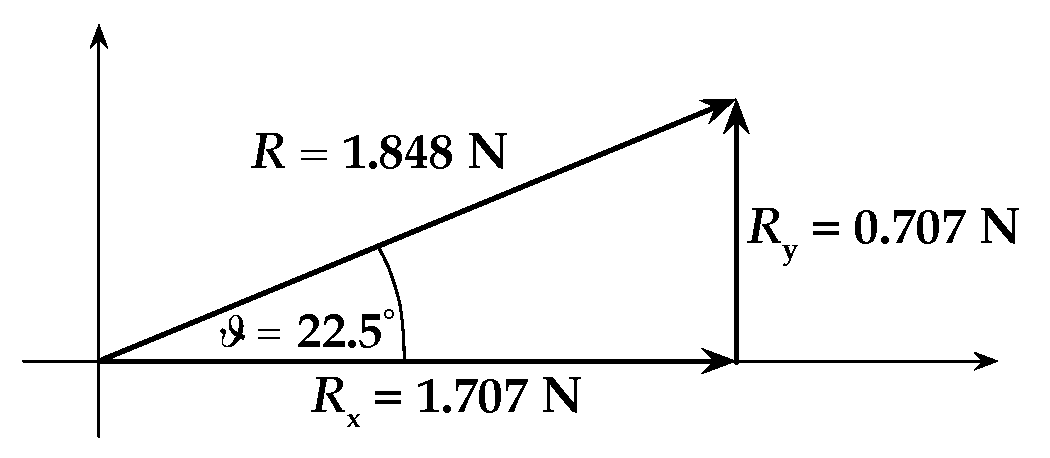
\includegraphics[width=3.5in]{Experiment01Figures/Figure04.pdf}
  \end{center}
  \caption{Example of $\vec{R}$, the sum of 2 vectors, illustrating $x$- and $y$-components, a well as its magnitude and angle with the $x$-axis.}
  \label{M01Fig04} 
\end{figure}



In this laboratory, an object will be presented with two known forces acting on it.  Equilibrium will be established by adding a third \textbf{equilibrant} force $\vec{F}_3$, such that the sum of the three forces is zero (at equilibrium). Thus, we must find the resultant $\vec{R}$ of the two given forces $\vec{F}_1$ and $\vec{F}_2$, and find the force $\vec{F}_3 = -\vec{R}$ --- equal in magnitude and opposite in direction to the resultant $\vec{R}$ of $\vec{F}_1$ and $\vec{F}_2$.  This is illustrated in Fig.~\ref{M01Fig05}.


%Figure05
\begin{figure}[h]
  \begin{center}
    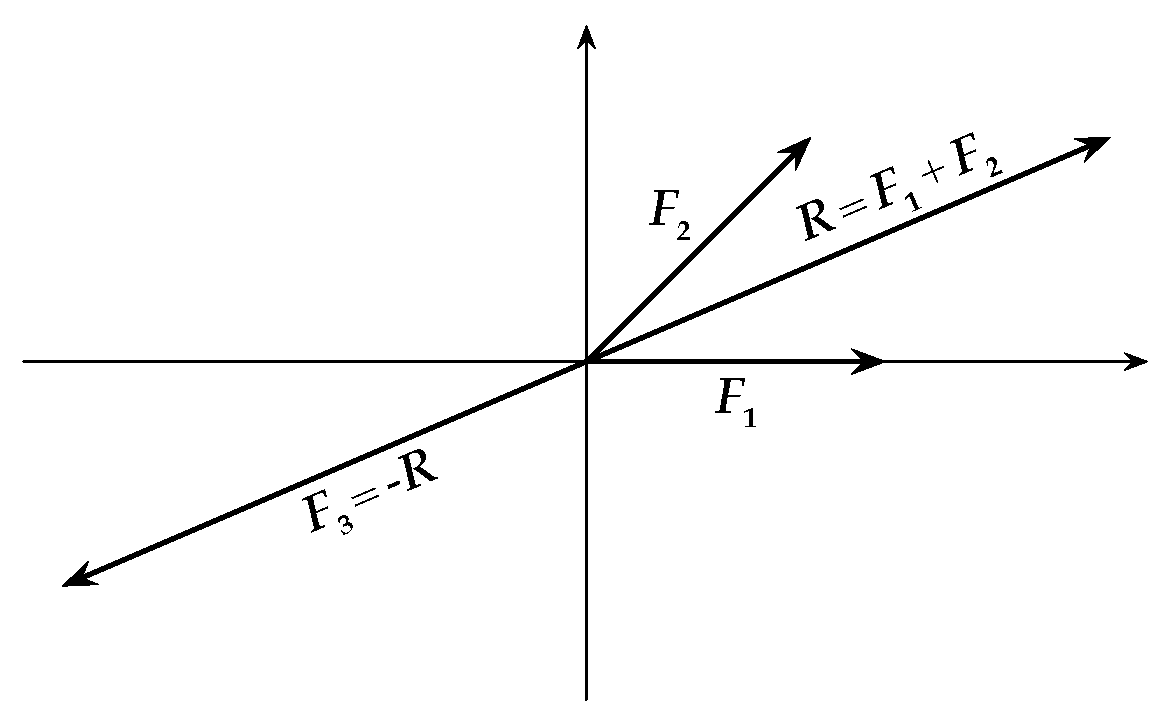
\includegraphics[width=3.6in]{Experiment01Figures/Figure05.pdf}
  \end{center}
  \caption{Illustration of the method to determine the force $\vec{F}_{3}$ needed to balance two given forces $\vec{F}_{1}$ and $\vec{F}_{2}$.}
  \label{M01Fig05}
\end{figure}

Here $\vec{F}_3$ is the equilibrant force necessary to equilibrate $\vec{F}_1$ and $\vec{F}_2$.  Note that, the resultant of $\vec{F}_1+\vec{F}_2+\vec{F}_3$ is zero since the ring is in equilibrium.

Force $\vec{F}_3$ has the same magnitude as the resultant $\vec{R}$, but acts in a direction opposite to $\vec{R}$ (recall that $\vec{R}=\vec{F}_1+\vec{F}_2$).  So we now have
\begin{equation}
  \vec{F}_3 = -\vec{R}.
\end{equation}
We conclude that the force necessary to equilibrate two or more forces is equal and opposite to the resultant of the two (or more) forces. This is additionally illustrated in an example of the force table apparatus we will use in Fig.~\ref{M01Fig06} right.





\underline{\textbf{Apparatus}}


%Figure05
\begin{figure}[h]
  \begin{center}
    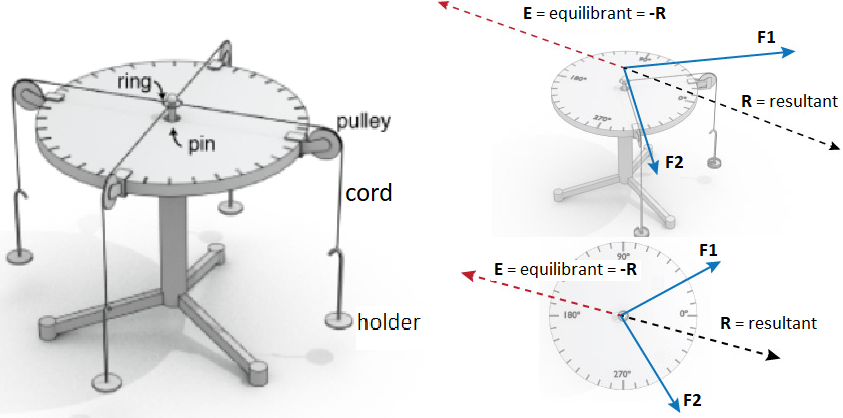
\includegraphics[width=5.5in]{Fall/Experiment01Figures/M1_ForceTable_06_table.png}
  \end{center}
  \caption{Illustration of the force table, and an example of to determine the force $\vec{F}_{3}$ needed to balance two given forces $\vec{F}_{1}$ and $\vec{F}_{2}$.}
  \label{M01Fig06}
\end{figure}

The apparatus for this experiment consist of a force table, weight holders, and weights (see Fig.~\ref{M01Fig06}).  The force table consists of a circular tabletop mounted on a vertical rod held in a tripod support with leveling screws.  The rim of the circular top has a $360\degree$ scale engraved on it along which it is possible to clamp a number of pulleys.  At the center of the table is a small ring held in place by means of a removable pin.  The ends of three cords are tied to the ring with each cord leading over a pulley and ending with a weight holder tied to its other end. When the forces along the cords acting upon the small ring are balanced, or in static equilibrium, the ring remains stationary. For this lab, the force pulling on the ring is the tension of the string, which is merely translated from horizontal on the table to vertical 


Each hanging mass has an associated weight (force) due to being pulled \textit{down} by gravity. This weight is balanced by the \textit{upward }tension force of the vertical part of the cord which is merely translated from vertical to horizontal tension by the pulley. Thus, the force pulling the ring in the direction of the cord is

\begin{equation}
  \label{eq:M01_ForceG}
  \vec{F_\text{weight}} = m \times \vec{g} = \vec{F_\text{tension}}
\end{equation}


For accurate measurements of the angles involved, each cord must be aimed directly at the center of the ring requiring that the equilibrium condition must be established when the ring is exactly centered around the pin on the table.



\section{Experimental Procedure}

\subsection{Preview}

For today's lab, two different cases will be assigned involving two given vectors and the \textbf{determination of the equilibrant vector}. A third case involves the \textbf{determination of the mass of two unlabeled masses} by balancing the system from a single known mass.% and changing the angles such that the angles are then assumed to be actual or true values (no uncertainty) system is balanced are the accepted values.

\underline{\textbf{Finding the Equilibrant (First two cases)}}


For each of the first two cases, you will have two given masses at given angles (direction).  Each mass, consisting of a $50\,\gram$ hanger plus the necessary additional mass, will be hung from a cord routed over a pulley at the assigned angular positions and finally tied to the ring.  A third cord, hanger, and pulley assembly is put in place for the third, unknown force vector.  Each force is the weight of the hanging mass at the pulley angle.  Determine the unknown forces for each of the two cases. % After you determine the unknown force in the third case, tilt the force table and determine any change in the third force with the tilted table.

If, for example, you are given the following case to work with
\[
\begin{array}{rll}
  \mbox{Mass \#1:} & 200\,\gram & \mbox{@}\,0\degree \\
  \mbox{Mass \#2:} & 250\,\gram & \mbox{@}\,135\degree.
\end{array}
\]
Place a pulley at $0\degree$ and add $150\,\gram$ to the $50\,\gram$ weight hanger for a total $200\,\gram$.  As mentioned in Eqn.~\ref{eq:M01_ForceG}, the tension on the cord is the same on both sides of the pulley so that the downward pull of gravity on the hanger and masses is equal to the tension in the cord leading to the ring.  Thus,
\[
\vec{F}_1 = m g = 0.20\,\kilo\gram\times 9.8\,\meter\per\second\squared
         = 1.96\,\newton\ @\ 0\degree.
\]
Similarly, add $200\,\gram$ to a $50\,\gram$ weight hanger and run its cord over a pulley mounted at $135\degree$.
\[
\vec{F}_2 = m g = 0.25\,\kilo\gram\times 9.8\,\metre\per\second\squared
         = 2.45\,\newton\ @ \ 135\degree.
\]

Having established the given magnitudes and directions for each of the given forces, $\vec{F}_{1}$ and $\vec{F}_{2}$, adjust both the amount of mass hanging on cord 3 and its angular position so that the ring is stationary at the center of the table.  In order for angular measurements to be accurate, \textbf{each cord must be on a line that crosses through the center of the table}.  Sighting \textit{along} each cord towards the center pin can help you to easily and accurately check this.

To determine the equilibrant vector $\vec{F}_{3}$, you will record both the angular position (\textbf{direction}) and total mass (to determine \textbf{magnitude} of the balancing force from the total hanging weight) required to balance $\vec{F}_{1}$ and $\vec{F}_{2}$.


\underline{\textbf{Determining 2 Unlabeled Masses (Third case)}}


In this case, you will experimentally \textbf{determine two unlabeled masses} by balancing the $x$ and $y$ components of the force of a known mass.
Place the pulley with the known mass $M_1 = 50\,\gram $ at $\theta_1 = 0\degree$.
Experimentally determine the angles $\theta_2$ and $\theta_3$ for the unlabeled masses $M_2$ and $M_3$ that result in the ring being in equilibrium. For this case, \textbf{assume angles $\theta_2$ and $\theta_3$ are actual values}.

%First find $M_2$ and $M_3$ using the graphical method.
%Accurately draw $ \vec{F}_1$ on graph paper using an appropriate scale.
%Draw a line in the direction of $\vec{F}_2$ at angle $\theta_2$ through the head of $\vec{F}_1$.
%Draw a line in the direction of $\vec{F}_3$ at angle $\theta_3$ through the tail of $\vec{F}_1$.
%Find the point where these two lines intersect to form a triangle representing equilibrium of the three forces.
%Determine the magnitude of $\vec{F}_2$ and $\vec{F}_3$ using your selected scale by measuring the sides of the triangle.
%Find the unknown masses by dividing by $g$.

We can calculate the theoretical unlabeled masses using the method of components.
You have to solve a pair of equations for the $x$ and $y$ components of force.
%This calculation is the algebraic version of finding the intersection of the two lines in the graphical method.
The equation for equilibrium in the $x$ direction is
\begin{equation}
  \label{eq:M01unknownx}
  (M_1 + M_2 \cos\theta_2 + M_3 \cos\theta_3)g = 0.
\end{equation}
The equation for equilibrium in the $y$ direction is
\begin{equation}
  \label{eq:M01unknowny}
  (M_2 \sin\theta_2 + M_3 \sin\theta_3)g = 0.
\end{equation}
$M_2$ is eliminated by multiplying the $x$ component by $\sin \theta_2$ and subtracting the $y$ component multiplied by $\cos \theta_2$
\begin{equation}
  \label{eq:M01solveM3}
  M_1 \sin \theta_2  + M_3 \cos \theta_3 \sin \theta_2 - M_3 \sin \theta_3 \cos \theta_2 = 0.
\end{equation}
Using the known values, solve for $M_3$ and enter the value in the table.

Similarly, eliminating $M_3$ gives
\begin{equation}
  \label{eq:M01solveM2}
  M_1 \sin \theta_3  + M_2 \cos \theta_2 \sin \theta_3 - M_2 \sin \theta_2 \cos \theta_3 = 0.
\end{equation}
Using the known values, solve for $M_2$ and enter the value in the table.

Measure $M_2$ and $M_3$ on the scale and enter the values in the table.










%Data analysis includes estimated or calculated errors. See the guidance starting at page \ref{sec:TypesErrors}.

It is good practice to \textbf{COMPLETE THE ANALYSIS OF THE FIRST CASE BEFORE CONTINUING TO THE NEXT CASE}. If you have some error in your experimental method or in your calculation, you can correct it before completing all the other cases. The layout of the data table for additional cases can then be created by copying the first case after you are confident in your results from the first case.


\subsection{CASE 1 \& 2 -- Finding the Equilibrant Vector (Balancing Force)}

\begin{enumerate}
\item \textbf{OVERALL GOALS:} 
\begin{itemize}
    \item Understand how to add and balance vectors using the \textbf{method of components}.
    \item Conduct 3 cases of two additive, known vectors (weights at given angles) to experimentally determine the third balancing or equilibrant vector.
    \item Compare the experimental results to theoretically expected vectors.
    \item \textbf{Assume} $0\degree$ is the $+x$ direction, $90 \degree$ is the $+y$ direction
\end{itemize}

\pagebreak

\item The first two cases are:
   % \begin{itemize}
  %      \item Case 1: 
  %      \begin{itemize}
  %          \item hanger 1: 150 g @ 0$\degree$
  %          \item hanger 2: 150 g @ 70$\degree$
  %          \item hanger 3: ? kg @ ?$\degree$
  %      \end{itemize}
  %      \item Case 2: 
  %      \begin{itemize}
  %          \item hanger 1: 100 g @ 75$\degree$
  %          \item hanger 2: 200 g @ 115$\degree$
  %          \item hanger 3: ? kg @ ?$\degree$
  %      \end{itemize}
  %      \item Case 3: 
  %      \begin{itemize}
  %          \item hanger 1: 150 g @ 120$\degree$
  %          \item hanger 2: 250 g @ 200$\degree$
  %          \item hanger 3: ? kg @ ?$\degree$
  %      \end{itemize}
  %  \end{itemize}

    \begin{tabular}{l|l}
    \textbf{Case 1:}     &  \hspace{20mm} \textbf{Case 2:} \\
    --- hanger 1: 150 g @ 0$\degree$    \hspace{20mm} & \hspace{20mm} --- hanger 1: 100 g @ 75$\degree$ \\
    --- hanger 2: 150 g @ 70$\degree$     & \hspace{20mm} --- hanger 2: 200 g @ 115$\degree$ \\
    --- hanger 3: ? kg @ ?$\degree$     & \hspace{20mm} --- hanger 3: ? kg @ ?$\degree$
    \end{tabular}

\item Create a data table for the first case. NOTE: The data layout for each of the first two cases is the same. Create for the first case and run the whole experiment, then you can copy/paste the same data table for the additional case(s).
%\item 
\begin{itemize}
    \item Common data section with accepted value of $g$ ($9.803\,\meter\per\second\squared$), mass of the hanger, and any other common values. You will reference these values in the calculations.
    \item With \textbf{three rows} (1 for each of the 3 vectors).% Also include additional \textbf{rows} for the average $g$ value, the $\pm$ uncertainty in gravity $\delta g$, the magnitude difference compared to the accepted $g$, \% diff. compared to the accepted $g$ \textit{DISCUSSION POINT for later}: How well does you average value of $g \pm \delta g$ agree with the accepted value of $g$?).
    \item Include \textbf{columns} for:
    \begin{itemize}
        \item $m_i$: hanging mass in kilograms (\kilo\gram)
        \item $\delta m_i$: your estimate of the experimental uncertainty [$\pm$ value] of the mass
        \item $F_i$: calculated magnitude of the force in Newtons (N) (see Eqn.~\ref{eq:M01_ForceG})
%        \item $\delta \vec{F}_i$: your derived experimental uncertainty of the magnitude of the force (e.g. $\delta \vec{F}_i = ((m_i + \delta m_i) \times \vec{g}) - ((m_i) \times \vec{g})$) where you are trying to make the final force value (due to $m_i + \delta m_i$) as large as possible to find the widest range of propagated uncertainty for a derived value
        \item $\theta_i$: direction of the force vector in degrees
        \item $\delta \theta_i$: your estimate of the experimental uncertainty of the angle
        \item $F_{i,x}$: calculated $x$-component of the force vectors (see Eqn.~\ref{Eq:M1_cosSinAngle}). Reminder, Excel needs angles in radians (use RADIANS() function to convert)
        %\item $\delta \vec{F}_x$: your derived uncertainty of the $x$-component, again trying to maximize the magnitude of the uncertainty (e.g $\delta \vec{F}_x = (\vec{F}_i + \delta \vec{F}_i) \times \cos{(\theta \pm \delta \theta)}$)
        \item $F_{i,y}$: calculated $y$-component of the force vectors
        %\item $\delta \vec{F}_y$: your derived uncertainty of the $y$-component in a similar manner (e.g $\delta \vec{F}_y = (\vec{F}_i + \delta \vec{F}_i) \times \sin{(\theta \pm \delta \theta)}$)
    \end{itemize} 
    \item Create a secondary table to analyze the results of your measurements. This is effectively one row as there would be just a single value for each of the variables. The columns should include variables:
     \begin{itemize}
        \item $\vec{R}_x$ \& $\vec{R}_y$: the $x$ and $y$ components of the resultant vector $\vec{R}$ of the two given force vectors $\vec{F}_1$ and $\vec{F}_2$
        \item $\vec{R}_\text{mag}$: magnitude of the resultant force vector in Newtons (see Pythagorean Theorem in Eqn.~\ref{Eq:M1_resultantMag})
        \item $\theta_{R}$: direction of the resultant in degrees (see Eqn.~\ref{Eq:M1_arctan} which stems from trigonometry). Use ATAN2() Excel function to get angle as measured counterclockwise from $0\degree$. Reminder, Excel returns angles in radians (use DEGREES() function to convert)

        \item $\vec{F}_{x,\text{total experimental}}$ \& $\vec{F}_{y,\text{total experimental}}$: the vector components of the measured total force, which is the vector sum of $\vec{R}$ and $\vec{F}_3$

        \item $\vec{F}_{mag,\text{total experimental}}$ (a.k.a. $\delta \vec{F}_3$): the magnitude of the total force, determined in similar fashion to Eqn.~\ref{Eq:M1_resultantMag}, but with $\vec{F}_{x,\text{total experimental}}$ \& \newline $\vec{F}_{y,\text{total experimental}}$. \textit{\textbf{Consider}}: The \textbf{total force should be zero} because the ring is in equilibrium. The magnitude of the total force is therefore a measure of the \textit{experimental uncertainty}. This effectively represents $\delta \vec{F}_3$ where your experimental result would be $\vec{F}_3 \pm \delta \vec{F}_3$.

        
        \item Based on your determined resultant $\vec{R}$
            \begin{itemize}
                \item $\vec{F}_{3,\text{theoretical}}$: your expected or theoretical magnitude of the equilibrant force in N
                \item $m_3,\text{theoretical}$: theoretical equilibrant mass in kg
%                \item $\delta m_{3,\text{theoretical}}$: uncertainty of $m_3,\text{theoretical}$ in kg as derived from 
                \item $\theta_{3,\text{theoretical}}$: theoretical equilibrant direction in deg. (e.g. $\theta_{R} + 180 \degree$)
            \end{itemize}
        
     


%        \item \% Difference between experimental Equilibrant force and theoretical
%        \item \% Difference between experimental Equilibrant direction and theoretical
    \end{itemize} 
\end{itemize}


    \item Starting with the first case, place the respective masses on hangers 1 \& 2
    \item Unscrew the black pulleys to rotate them around the tabletop to their given angles
    \item With hanger 3, add or subtract masses and scoot the pulley around the table until the ring is as perfectly centered around the center pin as possible to argue equilibrium
    \item Note your $m_3$ \& $\theta_3$ values. Also note your estimated uncertainties $\delta m_i$ \& $\delta \theta_i$
    \item Derive the hangers' respective forces (e.g. Eqn~\ref{eq:M01_ForceG})
    \item Determine the hangers' respective $x$ and $y$ components
    \item Determine the resultant $\vec{R}$ from your derived values for $\vec{R}_x$, $\vec{R}_y$
    \item Determine the resultant's angle $\theta_R$
    \item COMPARE your experimental results of hanger 3 to the theoretical values. Does $\vec{F}_3 \pm \delta \vec{F}_3$ overlap (and therefore agree) with your theoretical value $\vec{F}_{3,\text{theoretical}}$? If not, are there significant issues that may be contributing to the discrepancy? Discuss with instructor if so. To be further discussed in Sec.~\ref{M1:Interpretation}
    \item Repeat for the second case
\end{enumerate}





\subsection{CASE 3 -- Determining 2 Unlabeled Masses}




\begin{enumerate}
\item \textbf{OVERALL GOALS:} 
\begin{itemize}
    \item Understand how to determine two unknown values of a 3 vector system using the \textbf{method of components}. 
    \item \textit{CONSIDER}: Each vector has two pieces of information, \textbf{magnitude} and \textbf{direction} --- how many pieces of information total do we have to work from?
    \item Determine the masses of two figurines (one is a black Pikachu, the other is a white corgi that can each sit on their respective hangers) by balancing the force vectors. Treat Pikachu-black as $m_2$ and the corgi-white as $m_3$.
    \item Compare the experimental results to actual masses as measured with a triple-beam balance.
    \item \textbf{Assume} the angles for both Pikachu and the corgi, once found, are treated as given values (so you only have two unknowns with two equations).
\end{itemize}

\item The third case is:
    \begin{itemize}
        \item hanger 1: \space\space\space\space\space\space\space\space\space\space\space\space\space\space\space\space\space50 g @ 0$\degree$
        \item hanger 2 (Pikachu-black): ? kg @ ?$\degree$ (angle treated as given once determined)
        \item hanger 3 (corgi-white): \space\space\space? kg @ ?$\degree$ (angle treated as given once determined)
    \end{itemize}

\item Create a data table for this case:
\begin{itemize}
    \item Common data section with the accepted value of $g$ ($9.803\,\meter\per\second\squared$), the mass of the hanger, actual values of the figurines to be determined later, and any other common values.
    \item $m_1$: Given mass will be just the hanger, so 50 $\gram$ (but record in \kilo\gram)
    \item $\theta_1$: Angle of 0\degree for the empty hanger
    \item $\vec{F}_{x,1}$ \& $\vec{F}_{y,1}$: $x$ and $y$ components of the known mass's force vector
    \item $\theta_{2,\text{Pikachu-black}}$ \& $\theta_{3,\text{corgi-white}}$: Experimentally determined direction of the force vector in degrees --- \textbf{treat as actual given values once you find equilibrium. You will use these to solve for the masses later.}
    \item $m_{2,\text{Pikachu-black}}$ \& $m_{3,\text{corgi-white}}$: the experimental values of $m_2$ and $m_3$ from Eqn.~\ref{eq:M01solveM3} and Eqn.~\ref{eq:M01solveM2}
    \item $m_{2,\text{Pikachu-black, actual}}$ \& $m_{3,\text{corgi-white, actual}}$: the values of $m_2$ and $m_3$ as measured on a triple-beam balance.
    \item \% Difference of $m_2$ and $m_3$ experimentally found values to the actual measured values (see Eqn.~\ref{M1:PercentDiff} in Sec.~\ref{M1:Interpretation}).
\end{itemize}



    \item Place the respective masses on there hangers, with $m_1$ set to 0\degree
    \item Unscrew the black pulleys to rotate them around the tabletop until you find equilibrium. You are only changing the angles of $\theta_{2,\text{Pikachu-black}}$ \& $\theta_{3,\text{corgi-white}}$. NO ADDITIONAL MASS IS REQUIRED.
    \item Once you've found equilibrium, note the $\theta_{2,\text{Pikachu-black}}$ \& $\theta_{3,\text{corgi-white}}$ values as actual values to use in later equations (i.e. as if they're given angles)
    \item Determine $m_{2,\text{Pikachu-black}}$ \& $m_{3,\text{corgi-white}}$ using Eqn.~\ref{eq:M01solveM3} and Eqn.~\ref{eq:M01solveM2}
    \item Using a triple-beam balance, measure directly the actual mass of $m_{2,\text{Pikachu-black, actual}}$ \& $m_{3,\text{corgi-white, actual}}$
    \item COMPARE your experimental results of each of the unlabeled masses to their actual values. Calculate the \% difference of $m_2$ and $m_3$ experimentally found values to the actual measured values. What may be contributing to a larger or smaller difference? To be further discussed in Sec.~\ref{M1:Interpretation}.

\end{enumerate}


Post-Lab Submission --- Interpretation of Results on next page $\xrightarrow{}$




\pagebreak

% Interpretation of Results
\section{Post-Lab Submission --- Interpretation of Results}
\label{M1:Interpretation}
\begin{itemize}

\item Make sure to submit your finalized data table (Excel sheet)
\item What is a vector?
\item Case 1 \& 2 (Finding Equilibrant):
\begin{itemize}
    \item Looking at your experiment, why do the two given masses not add up to the third mass?
    \item What are the uncertainties of Experiment 1?
    \item What are your results, and how do they compare to the theoretical predictions?
        \begin{itemize}
        \item In other words, for each of the first two cases, COMPARE your experimental results of hanger 3 to the theoretical values for hanger 3.
            \begin{itemize}
            \item Does $\vec{F}_3 \pm \delta \vec{F}_3$ overlap (and therefore agree) with your theoretical value $\vec{F}_{3,\text{theoretical}}$? 
            \item Does $m_3 \pm \delta m_3$ overlap with your theoretical value $m_{3,\text{theoretical}}$?
            \item Does $\theta_3 \pm \delta \theta_3$ overlap with your theoretical value $\theta_{3,\text{theoretical}}$?
            \end{itemize}
        \end{itemize}
%    \item Does $\vec{F}_{mag,\text{total experimental}}$ actually equal zero?
    \item How does adding a few grams (i.e. $m_3 + \delta m_3$) change your results for $\vec{F}_3$?
    \item How does changing the angle (i.e. $\theta_3 \pm \delta \theta_3$) change your results $\vec{F}_3$?
\end{itemize}

\item Case 3 (Unlabeled Masses):
\begin{itemize}
    \item How do your values for $m_\text{Pikachu-black}$ and $m_\text{corgi-white}$ compare to your actual values from the triple-beam-balance?
    \item What is the percent difference between your experimentally determine masses and their actual measured values? Calculate the \% difference in each of the masses using the following relation:
	\begin{align} %
        \label{M1:PercentDiff}
	\mbox{\% Difference} = \frac{\mbox{Experimental} \ \mbox{Value} - \mbox{Actual} \ \mbox{Value}}{\mbox{Actual} \ \mbox{Value}} \times 100\%.
	\end{align}
    \item What uncertainties might make this difference larger or smaller?
\end{itemize}
\item What is the precision of your equipment (force table, masses, etc.)?
\item What are possible systematic errors of the experiment?




    
%\item[$\triangleright$] Find the resultant force for each of the three experimental cases. Using the method of components, find the magnitude and direction of this resultant $\vec{R}$.  The balancing force $\vec{F}_{3}$ equals the negative of resultant $\vec{R}$ of $ \vec{F}_{1}$ and $\vec{F}_{2}$, i.e.\ the direction of $\vec{F}_{3}$ is $180\degree$ from $\vec{R}$.
%%\item[$\triangleright$] For one of the cases, plot the vectors $\vec{F}_{1}$ and $\vec{F}_{2}$.  Graphically construct and draw the vector $\vec{R}$.  From $\vec{R}$, construct the expected $\vec{F}_{3}$.  On the same graph, plot your experimentally determined vector $\vec{F}_{3}$ and compare the two $\vec{F}_{3}$ vectors.
%          Calculate the \% difference in the magnitudes of the two vectors using the following relation:
%	\begin{align} %
%	\mbox{\% Difference} = \frac{\mbox{Experimental} \ \mbox{Value} - \mbox{Calculated} \ \mbox{Value}}{\mbox{Calculated} \ \mbox{Value}} \times 100\%.
%	\end{align}
%\item[$\triangleright$] Discuss in your lab report any discrepancy in the directions of the two vectors as well as their magnitude.
%%\item[$\triangleright$] Assume the force table is not level while you perform the experiment. Discuss the effect this would have on the outcome of your measurement of the equilibrium force $\vec{F}_{3}$. To determine this, tilt the balanced force table for one of the cases. Discuss the outcome among yourselves and with your lab instructor.
\end{itemize}

